\bab{BAB I}{Umum}

% ─────────────────────────────────────────────────────────────
\subsection{Tabel Kontribusi}

\begin{center}
\begin{tabularx}{\textwidth}{|c|p{4.2cm}|c|X|}
\hline
\textbf{No} & \textbf{Nama} & \textbf{NIM} & \textbf{Peran pada Milestone 2}\\ \hline
1 & Theo Kurniady & 13523154 & P3 inti (kebijakan skema, \textit{dead-letter queue}, \textit{replay}), P4 (Feed Satelit $\rightarrow$ WILDFIRE), Observabilitas (metrik, \textit{tracing}, dashboard)\\ \hline
2 & Hasri Fayadh Muqaffa & 13523156 & Platform Kubernetes (k3s, manifest, Secret, NetworkPolicy, \textit{one-command deploy}, Tester Agent), P2 uji beban (10.000 VU, \textit{scaling}, \textit{rolling update}), P3 laporan Tim Lapangan, P5 (Sensor Pantai, ketahanan, SLO, \textit{game day})\\ \hline
3 & I Made Wiweka Putera & 13523160 & P1 (penyimpanan terdistribusi, Audit API, dashboard analitik), P2 inti (\textit{leader election}, \textit{fencing token}, pengambilan tepat sekali)\\ \hline
\end{tabularx}
\end{center}

% ─────────────────────────────────────────────────────────────
\subsection{Deskripsi Umum Sistem}

Platform Koordinasi Kebencanaan BNPB adalah sistem terdistribusi yang menjadi hub koordinasi pusat penanggulangan bencana. Sistem mengintegrasikan data dari instansi sumber eksternal (BMKG untuk gempa dan tsunami, PVMBG untuk gunung api) serta, mulai Milestone 2, dari Feed Satelit (titik panas VIIRS) dan Sensor Pantai (anomali muka laut dan tinggi gelombang). Data tersebut distandarkan ke format kanonik tunggal (\textit{HazardEvent}), disimpan pada penyimpanan terdistribusi, lalu didistribusikan secara asinkron ke konsumen melalui NATS JetStream.

Pada Milestone 2, cakupan sistem diperluas menjadi:
\begin{enumerate}[label=\alph*.]
\item \textbf{Penyimpanan Terdistribusi (P1):} \textit{canonical store} berpindah dari satu PostgreSQL ke klaster CockroachDB 4 node dengan replikasi \textit{RF}=3 dan 8 \textit{hash shard} logis. Pembacaan lintas \textit{shard} memakai \textit{scatter-gather} dan menandai jawaban yang tidak lengkap (\kode{partial: true}).
\item \textbf{Aggregator Ketersediaan Tinggi (P2):} tiga atau lebih instance Aggregator di belakang satu Service. Hanya satu \textit{leader} yang mengambil data (\textit{lease} di basis data dengan waktu dari CockroachDB), dan setiap penulisan dilindungi \textit{fencing token}.
\item \textbf{Perubahan Skema dan Laporan Lapangan (P3):} perubahan skema yang tidak kompatibel disimpan utuh di \textit{dead-letter queue} untuk diproses ulang. Tim Lapangan mendapat jalur tulis \kode{POST /field-reports} yang membalas 202 hanya setelah laporan tersimpan di JetStream.
\item \textbf{Pemrosesan Aliran Satelit (P4):} \kode{satellite-ingestor} membaca aliran SSE, mengelompokkan deteksi menjadi kebakaran berdasarkan waktu deteksi, dan menyimpan \textit{offset} secara atomik bersama keadaan.
\item \textbf{Sumber yang Tidak Andal (P5):} \kode{sensor-pantai-poller} memvalidasi kontrak, memasang \textit{circuit breaker}, \textit{bulkhead}, \textit{retry} dengan \textit{jitter}, jalur prioritas untuk peringatan kritis, dan \textit{load shedding} berprioritas pada client-api.
\item \textbf{Platform dan Observabilitas:} seluruh komponen berjalan di Kubernetes (k3s, 2 node berkernel terpisah) dengan Prometheus, Grafana, dan Jaeger (OpenTelemetry).
\end{enumerate}

% ─────────────────────────────────────────────────────────────
\subsection{Diagram Arsitektur Sistem}

\gambarplaceholder{Diagram arsitektur sistem Milestone 2 (komponen, jalur data sinkron/asinkron, batas kepemilikan storage)}{7cm}
\isi{Ganti dengan gambar diagram arsitektur M2 (perbarui \kode{AAT\_M1\_Diagram-Arsitektur.png}).}

\textbf{Batas layanan dan kepemilikan storage.}
\begin{itemize}
\item \textbf{Sumber:} \kode{bmkg-mock}, \kode{pvmbg-mock}, Sensor Pantai (image asisten, berjalan di klaster), dan Feed Satelit (layanan asisten di luar klaster).
\item \textbf{Ingest:} \kode{aggregator} (BMKG/PVMBG, \textit{leader-only}) memiliki \kode{canonical-store} (CockroachDB). \kode{satellite-ingestor} memiliki \kode{satellite-store} (PostgreSQL). \kode{sensor-pantai-poller} tidak memiliki storage (cursor di JetStream KV). Sumber non-aggregator mengirim \kode{IngestMessage} ke \kode{hazard.ingest.<SOURCE>}; hanya Aggregator yang menulis ke \textit{canonical store}.
\item \textbf{Edge dan autentikasi:} \kode{token-service} memiliki \kode{token-db}; \kode{client-api} adalah satu-satunya pintu masuk client (JWT ES256, proyeksi \textit{scope}, \textit{rate limit}, \textit{load shedding}, \kode{POST /field-reports}).
\item \textbf{Distribusi event:} \kode{nats-jetstream} dengan stream \kode{BNPB\_EVENTS}, \kode{HAZARD\_INGEST}, \kode{FIELD\_REPORTS}, \kode{BNPB\_ALERTS}; konsumen \kode{notification-consumer}, \kode{audit-consumer}, \kode{field-report-consumer}; penerima simulasi \kode{stub-sink}.
\end{itemize}

\textbf{Alur data.} Jalur baca client bersifat sinkron (client-api $\rightarrow$ Aggregator $\rightarrow$ CockroachDB). Seluruh ingest dari sumber baru, distribusi event, laporan lapangan, dan peringatan kritis bersifat asinkron melalui JetStream dengan \textit{message ID} untuk deduplikasi.

% ─────────────────────────────────────────────────────────────
\subsection{Diagram Deployment}

\gambarplaceholder{Diagram deployment: penempatan komponen pada Node A dan Node B serta jalur data antar-node}{8cm}
\isi{Ganti dengan diagram final berdasarkan \kode{kubectl get pods -o wide -L role} pada klaster demo.}

\begin{center}
\begin{tabularx}{\textwidth}{|p{4.3cm}|p{3.2cm}|X|}
\hline
\textbf{Komponen} & \textbf{Penempatan} & \textbf{Alasan}\\ \hline
\kode{canonical-store} (4 pod) & Tersebar di kedua node & Data direplikasi Raft (\textit{RF}=3); pada topologi 2 node, 2 dari 3 replika setiap \textit{range} disematkan ke node \textit{control plane} agar kuorum bertahan saat node worker hilang\\ \hline
\kode{aggregator} (3 pod), \kode{token-service}, \kode{client-api} (2 pod) & Tersebar (\textit{soft anti-affinity}) & \textit{Stateless}; kehilangan satu node hanya mengurangi replika\\ \hline
\kode{token-db}, \kode{satellite-store}, \kode{nats-jetstream}, \kode{notification-consumer}, \kode{audit-consumer}, \kode{field-report-consumer}, \kode{prometheus} & Disematkan ke node \textit{control plane} (\kode{nodeSelector}) & Satu instance dengan data di disk node (\kode{hostPath}); skenario node mati hanya menyasar node worker\\ \hline
Mock, \kode{stub-sink}, \kode{satellite-ingestor}, \kode{sensor-pantai}, \kode{sensor-pantai-poller}, Grafana, Jaeger & Bebas & \textit{Stateless} atau keadaannya ada di storage/JetStream\\ \hline
\end{tabularx}
\end{center}

Jalur data antar-node: client-api $\rightarrow$ Service \kode{aggregator}; Aggregator $\rightarrow$ CockroachDB (DSN multi-host) dan replikasi Raft antar-pod CockroachDB; seluruh produsen/konsumen $\rightarrow$ NATS (Node A); Prometheus men-\textit{scrape} pod di kedua node; \textit{trace} OTLP $\rightarrow$ Jaeger.

% ─────────────────────────────────────────────────────────────
\subsection{Daftar Teknologi Terpilih}

Teknologi M1 (Go, NATS JetStream, bbolt, JWT ES256 + JWKS, \kode{x/time/rate}, zerolog, k6, Docker \textit{distroless}) tetap dipakai. Tambahan pada M2:

\begin{longtable}{|p{3.3cm}|p{3.4cm}|p{8.2cm}|}
\hline
\textbf{Komponen} & \textbf{Teknologi} & \textbf{Alasan Pemilihan}\\ \hline \endhead
Orkestrasi & k3s + Kustomize & Distribusi Kubernetes ringan untuk 2 VM; Kustomize (bawaan \kode{kubectl}) cukup untuk \textit{base} + \textit{overlay} topologi tanpa \textit{templating} tambahan. NetworkPolicy ditegakkan oleh pengendali bawaan k3s.\\ \hline
Penyimpanan kanonik & CockroachDB v24.1.6 & SQL terdistribusi dengan replikasi Raft, \textit{rebalancing} otomatis saat node datang/pergi, transaksi \textit{serializable}, dan HLC \kode{now()} sebagai sumber waktu \textit{lease}. Kompatibel dengan driver \kode{pgx} yang sudah dipakai.\\ \hline
Penyimpanan satelit & PostgreSQL 16 & Satu transaksi untuk deteksi, kebakaran, \textit{offset}, dan \textit{outbox} (pemrosesan tepat-sekali secara efektif).\\ \hline
Keadaan poller sensor & NATS JetStream KV & Cursor dan status Sensor Pantai tanpa menambah storage baru; durable dan terbaca client-api.\\ \hline
Metrik & Prometheus v2.55 & Penemuan pod lewat anotasi (\kode{kubernetes\_sd}), sehingga replika baru otomatis di-\textit{scrape}.\\ \hline
Dashboard metrik & Grafana 11 & Dashboard ter-\textit{provision} dari repositori (Services, Aggregator, Satellite, Coastal \& SLO).\\ \hline
\textit{Tracing} & OpenTelemetry + Jaeger & Satu \textit{trace} lintas client-api $\rightarrow$ Aggregator $\rightarrow$ CockroachDB dan lintas JetStream; \kode{trace\_id} di log.\\ \hline
Dashboard analitik & Chart.js (tertanam) & Halaman statis yang disajikan Aggregator (\kode{/analytics/}) tanpa CDN eksternal.\\ \hline
Uji beban & k6 (di luar klaster) & Skenario \textit{ramping} 10.000 VU dengan \textit{threshold} per fase.\\ \hline
\end{longtable}

% ─────────────────────────────────────────────────────────────
\subsection{Asumsi}

\begin{enumerate}[label=\alph*.]
\item Asumsi M1 tentang otonomi instansi sumber, \textit{eventual consistency} pada jalur baca client, otorisasi berbasis \textit{scope}, dan semantik \textit{at-least-once} pada broker tetap berlaku.
\item Skenario node mati hanya dikenakan pada node worker (topologi 2 node), sesuai ketentuan platform.
\item Feed Satelit dan Sensor Pantai berjalan pada waktu virtual yang dipercepat (60$\times$); seluruh logika waktu memakai jam sumber (\kode{acq\_date/acq\_time}, \kode{generated\_at}), bukan jam BNPB.
\item Sensor Pantai dan Feed Satelit adalah kotak hitam; kelompok hanya berinteraksi melalui kontraknya dan tidak bergantung pada ID, \textit{seed}, atau pola profil latihan.
\item Satu broker NATS (R1) dianggap memadai untuk prototipe; risikonya dibahas pada batasan P3 dan P5.
\item \isi{asumsi tambahan dari anggota lain bila ada}
\end{enumerate}

% ─────────────────────────────────────────────────────────────
\subsection{Perubahan dari Milestone 1}

\begin{longtable}{|p{4.4cm}|p{2.3cm}|p{8.2cm}|}
\hline
\textbf{Keputusan M1} & \textbf{Status} & \textbf{Alasan}\\ \hline \endhead
Docker Compose di satu mesin & Diubah & Seluruh komponen berjalan di k3s 2 node; Compose tetap dipakai untuk pengembangan.\\ \hline
\textit{Canonical store} satu PostgreSQL (JSONB) & Diubah & CockroachDB 4 node \textit{RF}=3 agar data tidak hilang bersama satu node dan beban tersebar (P1).\\ \hline
Satu Aggregator, semua instance melakukan \textit{polling} & Diubah & $\ge$3 instance dengan satu \textit{leader} dan \textit{fencing token} (P2).\\ \hline
\textit{Tolerant reader} hanya untuk perubahan aditif & Dipertahankan + diperluas & Perubahan aditif tetap diterima; perubahan tidak kompatibel disimpan di DLQ dan dapat di-\textit{replay} (P3).\\ \hline
Isolasi storage lewat jaringan Docker & Diubah & Ditegakkan dengan NetworkPolicy per storage.\\ \hline
Kredensial di \kode{.env} & Dipertahankan untuk pengembangan & Di klaster menjadi Secret per service + ConfigMap.\\ \hline
JWT ES256, proyeksi \textit{scope}, \textit{rate limit} per client & Dipertahankan & Ditambah \textit{load shedding} berprioritas berbasis kapasitas (P5).\\ \hline
client-api hanya baca & Diubah & Jalur tulis \kode{POST /field-reports} (P3).\\ \hline
Filter \kode{type} hanya SEISMIC/VOLCANIC, \kode{hazard\_id} UUID & Diubah & Seluruh tipe kontrak (termasuk WILDFIRE, COASTAL), ID kanonik \kode{hz-\ldots}, \textit{cursor pagination} diteruskan.\\ \hline
Satu durable consumer notifikasi & Diubah & Consumer kedua untuk stream prioritas \kode{BNPB\_ALERTS} (P5).\\ \hline
Log JSON + \kode{X-Correlation-ID} & Dipertahankan + diperluas & Ditambah metrik Prometheus, \textit{tracing} OpenTelemetry, dan \kode{trace\_id} di log.\\ \hline
Uji beban 50 VU & Diubah & 10.000 VU dijalankan dari luar klaster (P2).\\ \hline
\isi{keputusan M1 lain yang dibatalkan, bila ada} & & \\ \hline
\end{longtable}

% ─────────────────────────────────────────────────────────────
\subsection{Deklarasi Topologi}

\begin{center}
\begin{tabularx}{\textwidth}{|p{1.5cm}|p{2.6cm}|p{1.7cm}|X|X|X|}
\hline
\textbf{Node} & \textbf{Peran} & \textbf{Jenis} & \textbf{Host fisik} & \textbf{CPU/RAM host} & \textbf{vCPU/RAM node}\\ \hline
node-a & control plane + worker & VM \isi{} & \isi{} & \isi{} & \isi{}\\ \hline
node-b & worker & VM \isi{} & \isi{} & \isi{} & \isi{}\\ \hline
\end{tabularx}
\end{center}

OS/kernel tiap node: \isi{output \kode{kubectl get nodes -o wide}}. Bukti kernel terpisah: \isi{output \kode{scripts/k8s/verify.sh} bagian 1 (boot ID berbeda per node)}.

% ─────────────────────────────────────────────────────────────
\subsection{Observabilitas}

\begin{itemize}
\item \textbf{Metrik:} setiap service Go memasang paket bersama \kode{observability/} (latensi, \textit{error rate}, \textit{throughput} per rute dan per panggilan keluar, metrik pesan JetStream). Prometheus di klaster menemukan pod lewat anotasi \kode{prometheus.io/*}; label \kode{instance} = nama pod, \kode{node} = node tempat pod berjalan.
\item \textbf{Dashboard Grafana (folder BNPB):} \textit{Services overview}; \textit{Aggregator, sources and dead-letter queue} (status sumber, \textit{leader}, DLQ, \textit{outbox}); \textit{Satellite fire feed} (lag, latensi ingest, deteksi terlambat); \textit{Coastal sensor and alert SLO} (\textit{breaker}, data ditolak, jalur peringatan, SLO, \textit{load shedding}).
\item \textbf{\textit{Tracing}:} OpenTelemetry SDK $\rightarrow$ Jaeger (OTLP/HTTP), konteks W3C \kode{traceparent}. Satu permintaan terlacak client-api $\rightarrow$ Aggregator $\rightarrow$ CockroachDB dengan durasi tiap langkah (setiap \textit{query} SQL menjadi \textit{span}). \textit{Trace} juga diteruskan lewat header pesan JetStream, sehingga \textit{publish} Aggregator $\rightarrow$ consumer $\rightarrow$ stub-sink dan kebakaran dari \kode{satellite-ingestor} $\rightarrow$ \textit{upsert} di Aggregator masing-masing tampil sebagai satu \textit{trace}. Semua \textit{trace} disimpan, kecuali \kode{satellite-ingestor} yang disampel 5\% karena volumenya.
\item \textbf{Log:} JSON terstruktur dengan \kode{correlation\_id} dan \kode{trace\_id}/\kode{span\_id} yang sama dengan Jaeger, sehingga \textit{trace} yang lambat dapat ditelusuri ke log-nya dan sebaliknya.
\item \textbf{Paket bersama \kode{observability/}:} \textit{middleware} HTTP (metrik dan \textit{span} server, \kode{X-Correlation-ID}), \textit{transport} klien HTTP, propagasi \textit{trace} lewat header NATS, \textit{tracer} pgx untuk \textit{query} SQL, dan \textit{hook} zerolog. Setiap service cukup memanggil \kode{observability.Init} dan membungkus \textit{handler} serta klien HTTP-nya.
\item \textbf{Status \textit{leader}:} metrik \kode{aggregator\_leader} diatur oleh \textit{hook promote/demote} pemilihan \textit{leader}, dan setiap replika Aggregator di-\textit{scrape} terpisah, sehingga dashboard menunjukkan tepat satu \textit{leader} dan perpindahannya saat \textit{failover}.
\end{itemize}

\begin{figure}[H]\centering
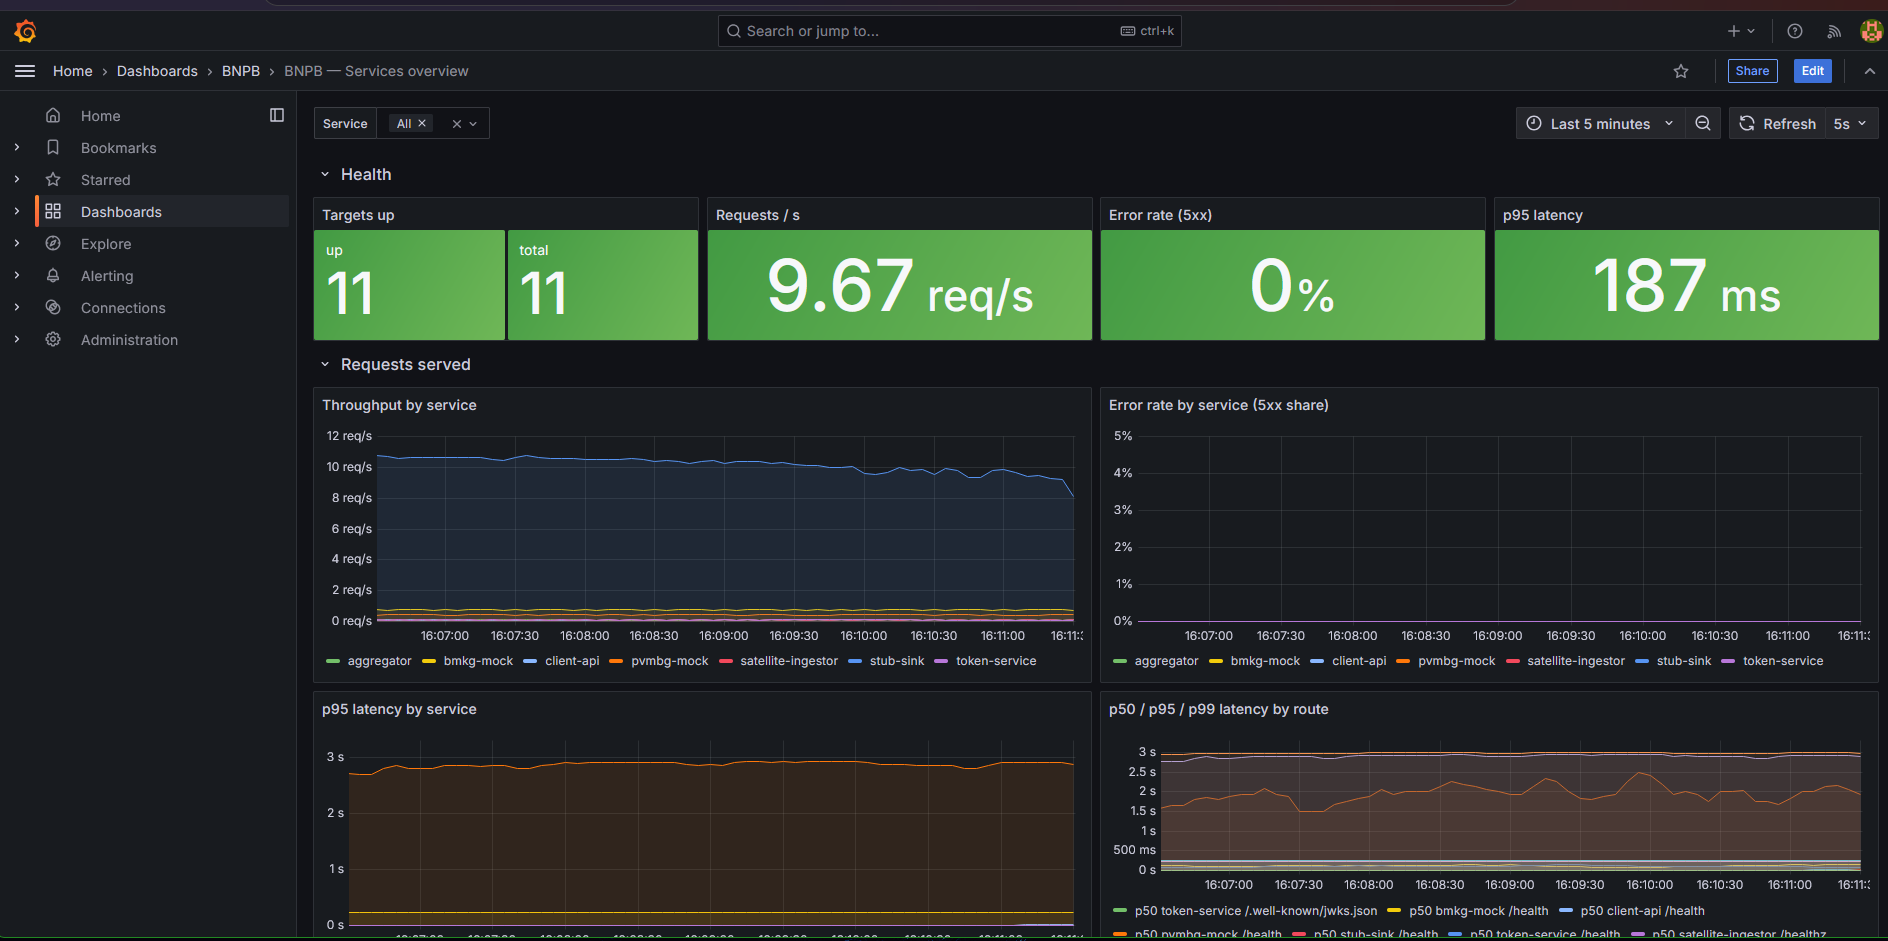
\includegraphics[width=\textwidth]{gambar/grafana-services.png}
\caption{Dashboard \textit{BNPB --- Services overview} (5 menit terakhir): 11 dari 11 target aktif, $\pm$9,7 permintaan/s, \textit{error rate} 5xx 0\%, dan p95 seluruh service 187 ms. Garis $\pm$2,9 s pada p95 per service adalah \kode{pvmbg-mock}, yang sengaja menunda setiap respons \kode{/volcanic-reports} 0,5--3 s untuk meniru sumber yang lambat.}
\end{figure}
\begin{figure}[H]\centering
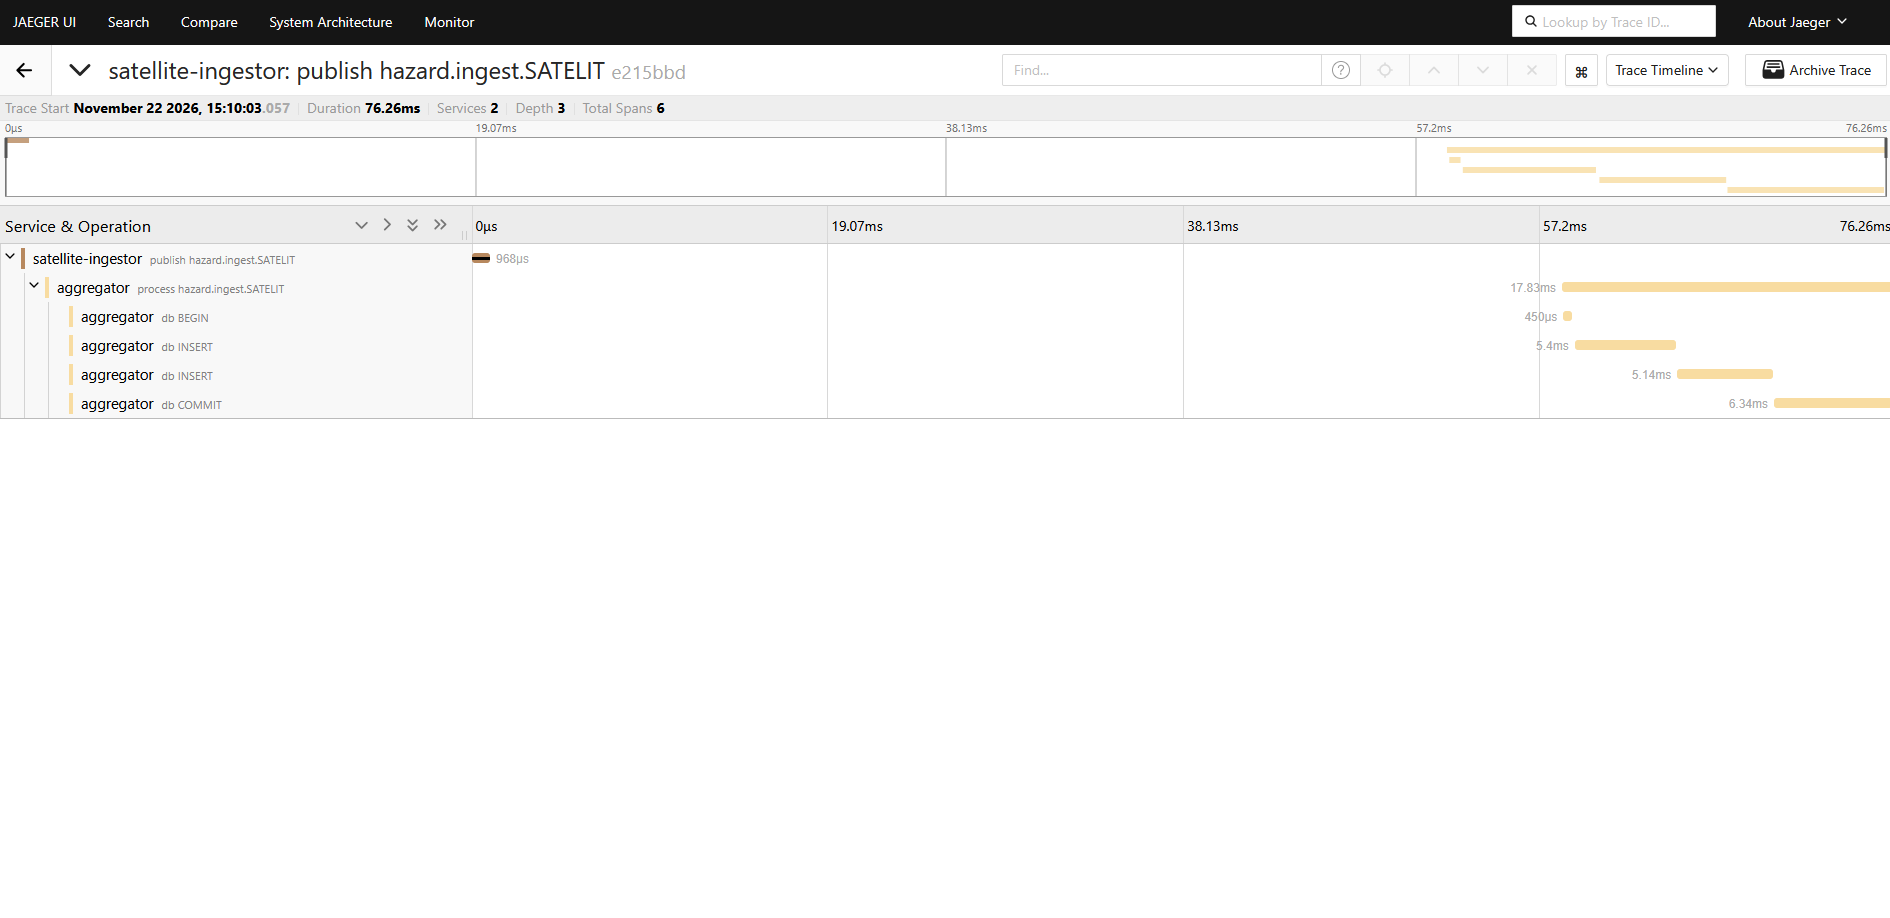
\includegraphics[width=\textwidth]{gambar/jaeger-trace.png}
\caption{Jejak satu pesan WILDFIRE lintas service di Jaeger: \kode{satellite-ingestor} mempublikasikan ke \kode{hazard.ingest.SATELIT} (0,97 ms), pesan menunggu di JetStream $\pm$57 ms, lalu Aggregator memprosesnya dalam satu transaksi CockroachDB (17,8 ms: \kode{BEGIN}, \kode{INSERT} ke \kode{canonical\_events}, \kode{INSERT} ke \textit{outbox}, \kode{COMMIT}). \textit{Trace context} diteruskan lewat header NATS.}
\end{figure}

% ─────────────────────────────────────────────────────────────
\subsection{Petunjuk Menjalankan Sistem}

Langkah lengkap ada pada \kode{README.md} bagian \textit{Kubernetes Deployment}.

\begin{enumerate}
\item \textbf{Menyiapkan klaster.} Dua VM Linux; Node A: \kode{curl -sfL https://get.k3s.io | sh -}; Node B bergabung dengan \kode{K3S\_URL} dan \kode{K3S\_TOKEN}. \kode{kubectl get nodes -o wide} menampilkan dua node \textit{Ready}.
\item \textbf{Konfigurasi.} \kode{cp .env.example .env}, isi kredensial (kunci ES256 via \kode{bash scripts/keys/gen-es256.sh}, token Feed Satelit, \kode{PANTAI\_AUTH\_TOKEN}, token audit).
\item \textbf{Deploy satu perintah:}
\begin{lstlisting}
K3S_NODES="<user>@<ip-node-a> <user>@<ip-node-b>" bash scripts/k8s/up.sh
\end{lstlisting}
Skrip membangun dan mengimpor image ke kedua node, membuat Secret, memuat dashboard Grafana, menerapkan \textit{overlay} \kode{two-node}, dan menunggu seluruh workload siap.
\item \textbf{Verifikasi platform:} \kode{bash scripts/k8s/verify.sh} (2 node berkernel terpisah, label \kode{role}, \textit{resources}, \kode{hostPath} untuk \kode{role=store}, NetworkPolicy, dan \textit{round trip} token $\rightarrow$ \kode{/v1/events}).
\item \textbf{Tester Agent:} \kode{bash scripts/k8s/tester-agent.sh install}, \kode{list}, \kode{practice <nama>}, \kode{logs}.
\item \textbf{Titik masuk:} client-api \kode{:30080}, token-service \kode{:30083}, mock \kode{:30081/:30082}, Grafana \kode{:30300}, Prometheus \kode{:30090}, Jaeger \kode{:30686}; Aggregator melalui \kode{kubectl port-forward svc/aggregator 8090:8090}.
\end{enumerate}
